\documentclass{article}%
\usepackage[T1]{fontenc}%
\usepackage[utf8]{inputenc}%
\usepackage{lmodern}%
\usepackage{textcomp}%
\usepackage{lastpage}%
\usepackage{authblk}%
\usepackage{graphicx}%
%
\title{High cellular organization of pyoverdine biosynthesis in Pseudomonas aeruginosa: clustering of PvdA at the old cell poleemi\_274}%
\author{Joanna Brandt}%
\affil{Priority Research Centre for Cancer Research, University of Newcastle, Callaghan, NSW, Australia}%
\date{01{-}01{-}2012}%
%
\begin{document}%
\normalsize%
\maketitle%
\section{Abstract}%
\label{sec:Abstract}%
A team of researchers from UCSF has identified specific molecular switches controlling the supply of cell{-}cell contact and decreased attack response in the breast cancer of a young woman with an extremely high expression of cells 1, the closest approximation to human breast cells.\newline%
The researchers report their findings in the December 28, 2011 issue of the journal PLoS ONE, describing the findings of the first study to combine genetics data with cancer research protocols into a multi{-}pronged approach to establish what influences the protein driving breast cancer cell spreads, and what changes will take place in breast cancer cells to catalyze these changes.\newline%
"Our previous work showed that giving more empathy to cells carried by these xenotransferase{-}specific blockers is linked to reduced risk of breast cancer cell spreads," says Dr. Malcolm Shen, professor of molecular oncology at UCSF and head of the multidisciplinary cancer research team at UCSF Chang{-}Ping Cancer Center. "Our work adds a new dimension to that understanding, identifying individual molecular switches in breast cancer that are actively changing the cell{-}cell interaction, stimulating the spread of cancer cells. And, while this is an exciting discovery, it is the first time that we have shown that the target switches for mTOR, a specific form of miR{-}165, have any impact on the formation of breast cancer cells in cellular living tissue."\newline%
This work, led by senior authors Jun Hsiao, MD, postdoctoral associate, and Koyie Fuk, PhD, associate professor of pathology, was supported by grants from the National Cancer Institute and the National Human Genome Research Institute (NHHRII), the oncology team of which also includes assistant postdoctoral associate, Dr. Kwok T. Kaixu, PhD, and Kim T. Kim, PhD, and a team of other UCSF researchers.\newline%
The research was conducted in a novel method in which a fluorescence imaging technique was used to study cells from this young woman. The new data provides evidence that mTOR disrupts the normal function of membrane transporters and adversely affects cell germ cell membranes, leading to increased cell invasion and the formation of cancer{-}like cell lines.\newline%
"A wide range of cell types have been studied through collaborative research and understanding to improve our understanding of how cell dynamics affect cancer and thus evaluate their role in potentially cancer{-}causing outcomes," says Henry Maurer, PhD, Director of the UCSF Institutes for Cancer Research, who led the research team. "Because our findings emphasize the possibility that mTOR is involved in the cell's ability to evolve normal ability to form breast cancer, our results will improve the understanding of how mTOR functions in the breast. Also, while mTOR is shown to be a basic constituent of all receptors, what we learned is that mTOR is a key component in the front end of that pathway. The health of human breast cells will be directly impacted by the molecular changes that this knowledge provides."\newline%
The diagnosis of breast cancer is 1 in 88 women in the United States, making it the leading cause of cancer death in U.S. women.\newline%
"Our results reinforce how early and robustly these parameters are important," notes lead author Prof. Zhu Chen, PhD, a graduate student in Nanning Huang, PhD's lab. "Early evidence identifies the molecular switches that shape how the breast develops and metastasizes."

%
\subsection{Image Analysis}%
\label{subsec:ImageAnalysis}%


\begin{figure}[h!]%
\centering%
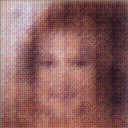
\includegraphics[width=150px]{500_fake_images/samples_5_408.png}%
\caption{A Man In A Tie Is Standing In A Room}%
\end{figure}

%
\end{document}